% !TEX root = main.tex
%%%%%%%%%%%%%%%%%%%%%%%%%%%%%%%%%%%%%%%%
%%%%%%%%%%%%%%%%%%%%%%%%%%%%%%%%%%%%%%%%
\section{\approach} \label{sec:t5}
%%%%%%%%%%%%%%%%%%%%%%%%%%%%%%%%%%%%%%%%
%%%%%%%%%%%%%%%%%%%%%%%%%%%%%%%%%%%%%%%%

\subsection{Learning to Generate Complete Log Statements}

\subsubsection{Text-to-Text-Transfer-Transformer (T5)}


The T5 model was introduced by Raffel \etal \cite{raffel2019exploring} to support multitask learning in the domain of NLP (Natural Language Processing). The novel idea behind the T5 model is to reframe NLP tasks in a unified text-to-text format in which the input and output are always text strings. For instance, a single model can be trained to translate across languages  (\eg learning the translation of sentences from English to French) and to autocomplete sentences. This approach is based on two phases: \textit{pre-training}, which allows defining a shared knowledge-base useful for a large class of sequence-to-sequence tasks, and \textit{fine-tuning}, which specializes the model to specific tasks of interest. 

\subsubsection{A peek under the hood}
T5 is based on the transformer model architecture that allows handling a variable-sized input using stacks of self-attention layers. When an input sequence is provided, it is mapped into a sequence of embeddings passed into the encoder. The T5, in particular, and a transformer model \cite{vaswani2017attention}, in general, offer two main advantages over other state-of-the-art models: (i) it is more efficient than RNNs since it allows to compute the output layers in parallel, and (ii) it is able to detect hidden and long-ranged dependencies among tokens, without assuming that nearest tokens are more related than distant ones. The latter, is particularly relevant in code-related tasks since a variable declaration may be distant from its usage. To this extent, the T5 model can relate the tokens representing the declaration of a local variable in the first statement of a method with the tokens implementing a return statement in which the value of such a variable is returned (despite the fact that the two statements could be far apart). 

In our work, we rely on the same T5 architecture (\ie T5$_{small}$) that has been exploit by Mastropaolo \etal \cite{mastropaolo2022using} to support the task of complete log statements generation. In this regard, the authors relied on such T5 variation because it allowed a reasonable trade-off between the training time needed to train a  60M parameters model (\ie T5$_{small}$)  and the results they were able to achieve.
 
Specifically, the T5\textsubscript{\textit{small}} architecture is characterized by six blocks for encoders and decoders. The feed-forward networks in each block consist of a dense layer with an output dimensionality ($d_{ff}$) of 2,048. The \textit{key} and \textit{value} matrices of all attention mechanisms have an inner dimensionality ($d_{kv}$) of 64, and all attention mechanisms have eight heads. All the other sub-layers and embeddings have a dimensionality ($d_{model}$) of 512. The code implementing the T5 model is publicly available in our replication package \cite{replication}.


\subsubsection{Pre-training Dataset}

To build the dataset, we used GHS (GitHub Search) the search tool by Dabic \emph{et al.} \cite{dabic2021sampling} that allows using tailored specifications to identify Github \cite{github} projects. Specifically, we used the same selection criteria used by Mastropaolo \etal \cite{mastropaolo2022using} in the work presenting LANCE.
In this regard, we selected all public non-forked \java projects with minimum 500 commits, 10 contributors, and 10 stars.
The selection criteria on the number of commits, contributors, and stars are necessary to avoid personal/toy projects, and 
by choosing non-forked repositories we reduced the chances to mine duplicated code. 
We collected 6,352 candidate projects of which we were able to clone the latest snapshot of 3,865 of them. 
We scanned all the cloned repositories to assess if a \texttt{POM} (Project Object Model)\footnote{A POM file is used in Maven to declare dependencies towards Maven libraries.} file or a \texttt{build.gradle}\footnote{A build.gradle file describes the build configuration, tasks, plugins and dependencies for a gradle project.} file was present in the projects' directory.
All the projects using a different build automation tool were discarded.
Whilst Mastropaolo \etal \cite{mastropaolo2022using} mined only Maven projects we decided to expand our search to Gradle projects to increase the chances of identifying new relevant data points.
To have an even more cohesive codebase we required the projects to have an explicit dependency on either Apache Log4J \cite{log4j}, a well known Java logging library, or on SLF4J (Simple Logging Facade for Java) \cite{slf4j}, an abstraction for Java logging frameworks similar to Log4J.
We found out that 2,978 of the cloned repositories had an explicit dependency on either Log4J or SLF4J. Afterwards, we leveraged srcML \cite{srcml} to extract all the \java methods from the selected projects. In details, we used the \java methods srcML representation to automatically remove all the inline comments, and to identify all the methods' log statements. We then filtered out all methods containing log statements with custom log levels (\emph{i.e.}, log levels different from \texttt{FATAL}, \texttt{ERROR}, \texttt{WARN}, \texttt{DEBUG}, \texttt{INFO}, and \texttt{TRACE}).
The purpose of this filtering was to remove all methods containing log statements with project ad-hoc log levels, thus that are not generalizable.
Then, we used \emph{javalang} \cite{javalang} to tokenize the methods obtaining the method representation as a flat stream of tokens.
Once we had the tokenized Java methods, we removed all the instances having $\#tokens < 10$ or $\#tokens \geq 512$, similar filtering has been done in previous works \cite{mastropaolo2021empirical,tufano2021automating,tufano2022using,ciniselli2021empirical, Tufano:tosem2019} to limit the computational expenses of training DL-based models.
To avoid methods overlapping between training, validation, and test datasets we also removed all the duplicates. 
Finally, we filtered out all the methods containing non-English characters to obtain an even more coherent codebase. 
To ensure the quality of the processed dataset we performed a manual analysis on a sample of 200 random methods. 
The purpose of such an analysis was threefold: (i) ensure  the dataset did not contain false-negative logs (\emph{i.e.}, log statements not identified during the creation of the dataset) (ii) ensure the dataset did not contain false-positive logs (\emph{i.e.}, pieces of code wrongly identified as log statements), and (iii), guarantee that all the instances were preprocessed correctly.
This left us with a dataset of 13,100,955 Java methods of which XXXX contain at least one log statement. We used 12,322,588 non-logged \java methods to build our pre-training dataset and XXXXX logged \java methods have been used to build the fine-tuning dataset as reported in Table \ref{tab:ds-summary-1}. 

\begin{table}[h]
	\centering
	\caption{Num. of methods in the datasets used in the differentiated replication of LANCE}
	\begin{tabular}{ccccccccc}
		\hline
		\multirow{2}{*}{\textit{\textbf{Dataset}}} & \multicolumn{2}{c}{\textbf{train}} & \textbf{} & \textbf{eval} & \textbf{} & \textbf{test}  \\ \cline{2-3} \cline{5-5} \cline{7-7} 
		& \textbf{w/ log} & \textbf{w/o log} & \textbf{} & \textbf{w/ log} & \textbf{} & \textbf{w/ log} \\ \hline
		\textit{pre-training dataset}              & -               &      12,332,588  &           & -               &           &  -               \\
		\textit{fine-tuning dataset}               & 253,501         & -                &           & 31,721          &           & 31,651          \\ \hline
	\end{tabular}
	\label{tab:ds-summary-1}
\end{table}



\begin{figure}[h!]
	\label{pre-training}
	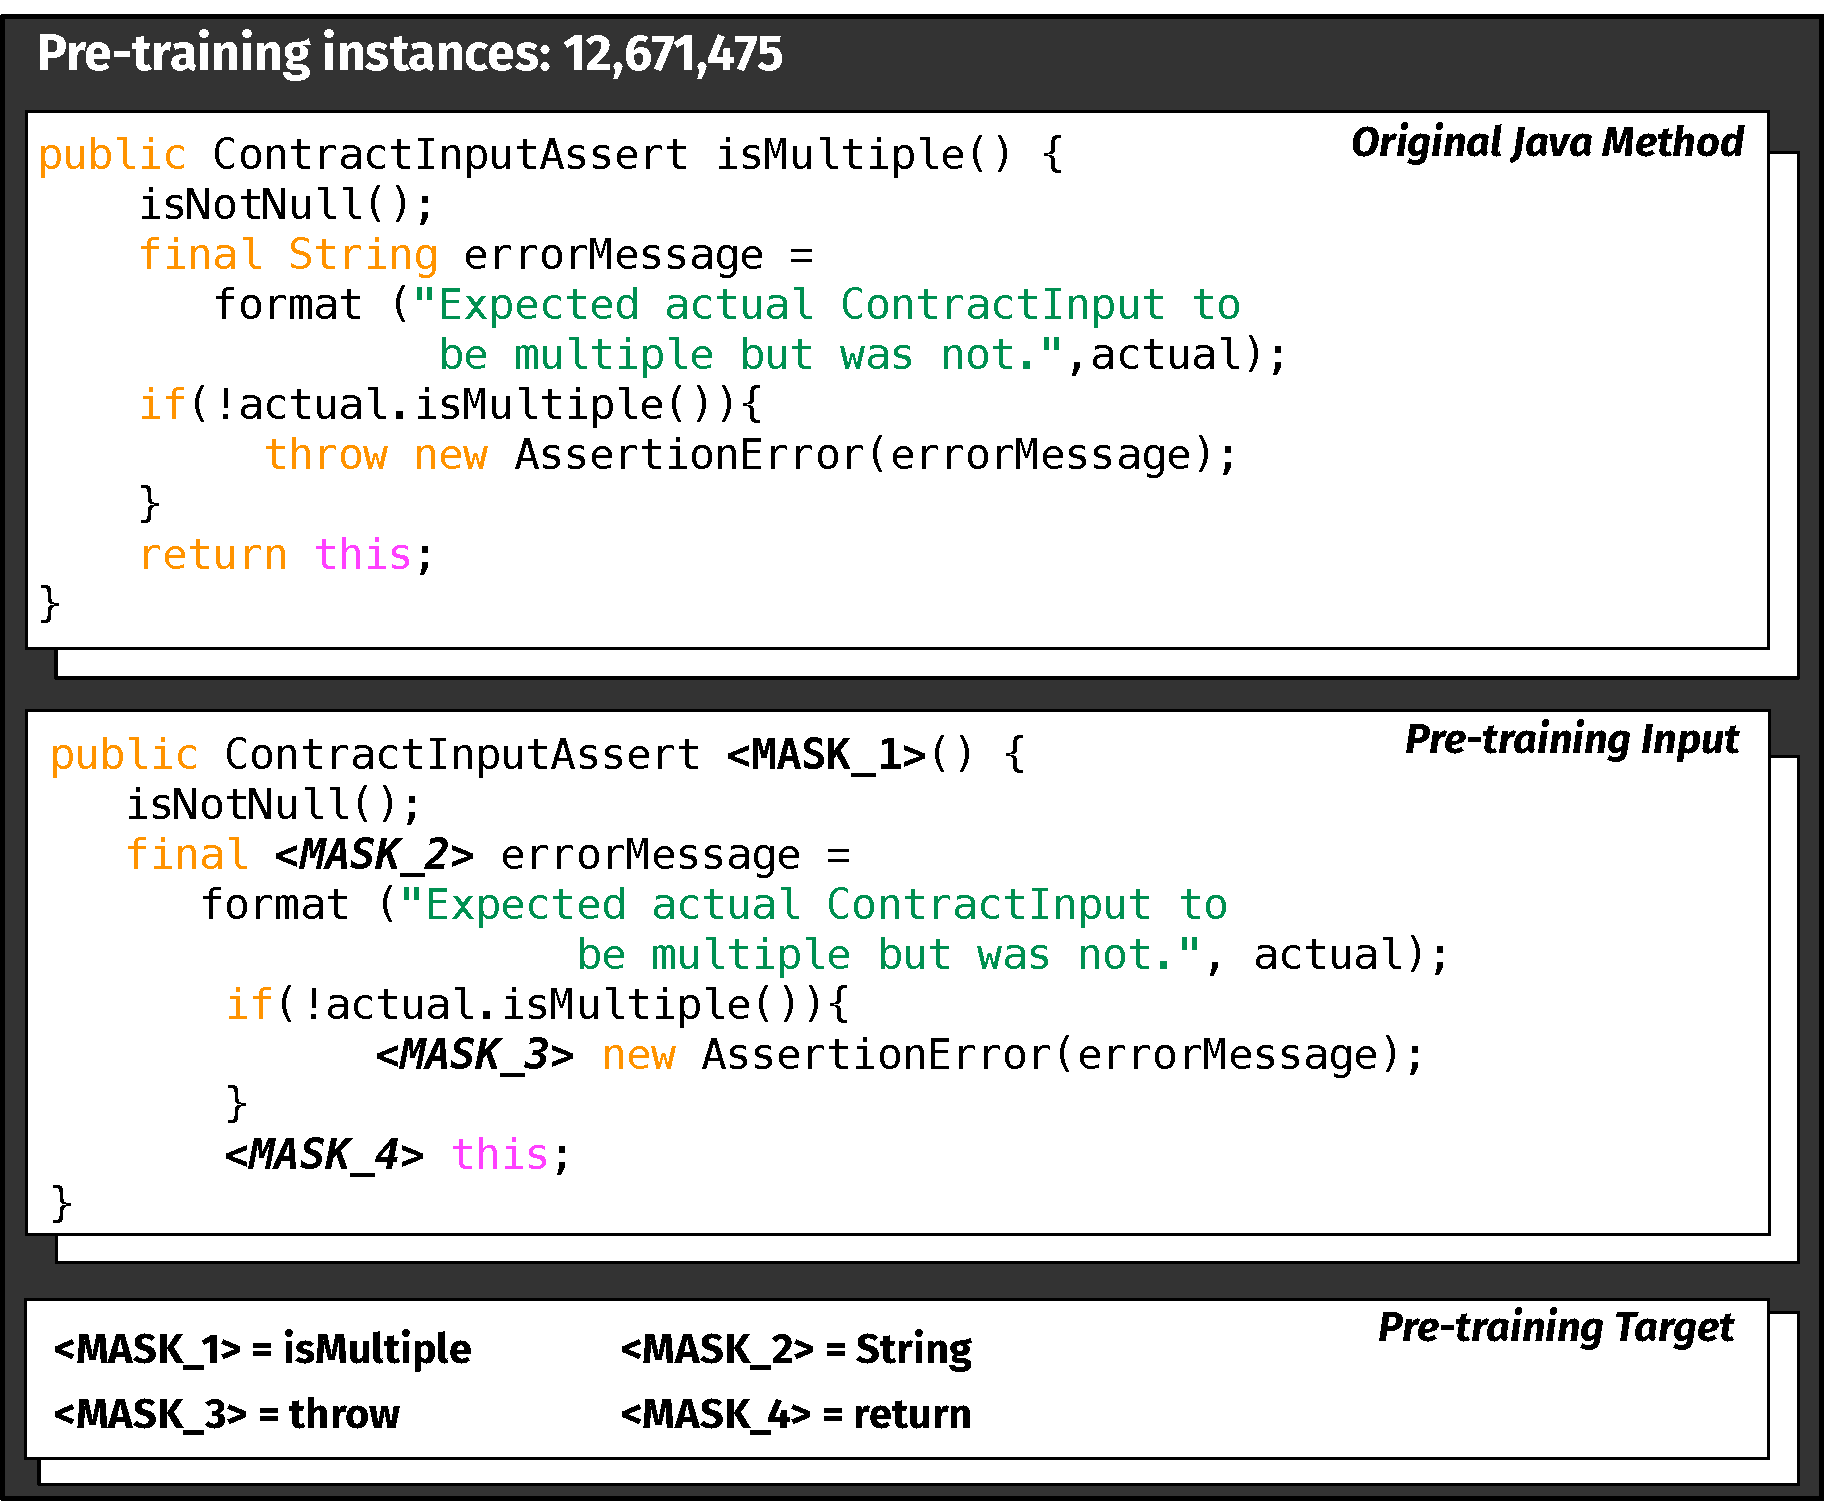
\includegraphics[width=\columnwidth]{img/pre-training.pdf}
	\caption{Example of pre-training instance.}
\end{figure}




\subsubsection{Fine-tuning Dataset}
To build the fine-tuning dataset that replicate what have been done by Mastropaolo \etal \cite{mastropaolo2022using}, we pre-process each training instance (\ie \java method in the training-set) by removing one log statement at a time from the \java method. This process, leaves us with a pair $<M_i, M_t>$ featured by the input and the target sequence in which $M_i$ represents the original \java method $M$ without the target log statement, while $M_t$ is the original \emph{Java} method equivalent to $M$. For those methods containing more than one log statement, we created $n$ pairs of input-target sequences, with $n$ being the number of log statements in the method. To ensure that after the log statement removal all the instances are still valid Java methods, we parsed each instance we created using JavaParser \cite{} and removed all the instances the tool was not able to parse or instances that after the instrumentation have been duplicated. Finally, the fine-tuning dataset replicating the approach implemented by Mastropaolo \etal \cite{mastropaolo2022using}, has been split into 80\% training, 10\% validation, and 10\% test. In \tabref{tab:} are reported the number of entries in each dataset. While the instances featuring the test set have been used to assess the performance of our model (\emph{i.e.}, its ability to generate complete log statements and inject them in the correct location, the validation set was used to find the best configuration of hyperparameters \secref{sec:training}. Later, we used the validation dataset also to perform early-stopping (Section \ref{t5-finetuning}) taming the over-fitting problem.

As described in \secref{sec:intro}, our multi-log injection approach is built on top of two separate models: (i) a classification model that predict whether a method requires or not log statements  and, (ii) the model performing the injection (if needed) within the \java method we provide as input.

For the latter (\ie multi-log injection model), the fine-tuning dataset has been built applying the following procedure: for each method featuring the 253,501 instances having logs, we chose an arbitrary number $k$ from 0 to $n$, where $n$ is the number of log statements in the method. Then, we randomly select $k$ log statements out of the method’s $n$ logs that are going to be removed. The resulting stream of tokens given by the pair $<M_i, M_t>$ represents one training instance that has been created starting from the method $M$, in which $M_i$ describes the model input sequence while $<M_t>$ being  the corresponding target sequence (\ie the method $M$ without log statements removed). For all those cases in which $k$ is equal to 0, no log statements will be removed and, thus, the input sequence and the target sequence are equal (i.e., the original \java method). 
Ultimately, we split the fine-tuning dataset into 80\% training, 10\% validation, and 10\% test. In \tabref{tab:} are reported the number of entries in each dataset.  

To build the dataset needed for predicting whether or not log statements are needed in a \java method, we use the same methods featuring the dataset built for the multi-log injection model. Specifically, starting from the original set of 253,501 \java methods having at least one log statement, we apply the same procedure described above with the only difference being the replacement of the target sequence with a binary choice either  \texttt{Need} or \texttt{No need}. Instances labeled as \texttt{No need} correspond to the entries that, in the previous dataset have the input sequence equal to the target sequence (\ie methods that already contain all the necessary log statements, thus need no further logs). On the other hand, the entries labeled as \texttt{Need} are those missing at least one log statement. It is possible that two methods differ only because a they contain a different log statements, if said statements are removed then the methods could be considered equal. Since in these specific datasets all the methods from which log statements have been removed point to the same target sequence (\ie \texttt{Need}), it is possible that duplicates have been created among training, validation, and test sets. Thus, eventually we removed all the between dataset duplicates and we obtained the datasets summarized in \tabref{tab:}



\subsubsection{Training and Hyperparameter Tuning} \label{sec:training}
In this section we outline how the pre-training and the fine-tuning phase have been conducted to support the task of complete log statements generation (\ie injection of log statements). Afterwards, we also outline how we found the best-performing model relying on two strategies: (i) hyperparameter tuning  and (ii) early stopping.

The goal of the pre-training phase is to teach the model generalizable knowledge that is useful for the downstream task. For the task we aim at supporting (\ie complete log statement generation), during the pre-training, the model gains basic knowledge of the \java language by learning the most recurrent patter characterizing \java. This is achieved by leveraging a specific pre-training objective, namely, MLM (Masked-Language-Modeling). Said objective consists in teaching the model to predict missing or masked tokens in the input. We processed the methods to obtain an input sequence in which 15\% of random tokens have been masked as depicted in \figref{fig:pre-training}.
We pre-train the T5 model for 500k steps on a dataset of 12,332,588 instances using Google Colab's 2x2, 8 cores TPU topology with a batch size of \highlight{YY} and a maximum sequence length of \highlight{ZZZ}. 
To create the input and target sequences to fine-tine the model, we took each instance of the fine-tuning dataset (\ie train, test and eval) and we removed one log statement. The corresponding target sequence is the complete Java method.
For those methods containing more than one log statement, we created \emph{n} pairs of input-target sequences, with \emph{n} being the number of log statements in the method.
For each one of the \emph{n} pairs, we removed a different log statement, since the target sequences of those pairs is the same we made sure that there were no duplicates between training, validation, and test datasets. 
To ensure that after the log statement removal all the instances are still valid Java methods, we parsed each instance of the three subsets (\emph{i.e.}, train, eval, and test) using JavaParser \cite{javaparser} and removed all the instances the tool was not able to parse.
In Table \ref{tab:ds-summary-1} are reported the actual number of methods in each dataset



Concerning the hyperparameters tuning phase, as discussed by Mastropaolo \etal \cite{mastropaolo2021studying}, we did not tune the T5 model hyperparameters during the pre-training phase, because such a phase is task-agnostic, and therefore it would provide limited benefits. Instead, we rely on the same strategy adopted by the same authors in \cite{mastropaolo2022using} when fine-tuning the hyperparameters of the model. Specifically, we experiment with four different learning rate scheduler: (i) \textit{Constant Learning Rate} (C-LR): the learning rate is fixed during the whole training (we use $LR = 0.001$, \ie the value used in the original paper \cite{raffel2019exploring}); (ii) \textit{Inverse Square Root Learning Rate} (ISR-LR): the learning rate decays as the inverse square root of the training step (the same used for pre-training by Raffel \etal); (iii) \textit{Slanted Triangular Learning Rate \cite{howard2018universal}} (ST-LR): the learning rate first linearly increases and then linearly decays to the starting learning rate;  (iv) \textit{Polynomial Decay Learning Rate} (PD-LR): the learning rate decays polynomially from an initial value to an ending value in the given decay steps. Table \ref{tab:learning-rates} reports all the parameters used for each scheduling strategy as did in \cite{mastropaolo2022using}.

\begin{table}[h]
	\centering
	\begin{tabular}{ll}
		\hline
		\textbf{Learning Rate Type} & \textbf{Parameters}               \\ \hline
		Constant                     & \textit{LR = 0.001}               \\
		Inverse Square Root         & \textit{LR\textsubscript{starting} = 0.01}  \\
		& \textit{Warmup = 10,000}          \\
		Slanted Triangular          & \textit{LR\textsubscript{starting} = 0.001} \\
		& \textit{LR\textsubscript{max} = 0.01}       \\
		& \textit{Ratio = 32}               \\
		& \textit{Cut = 0.1}                \\
		Polynomial Decay            & \textit{LR\textsubscript{starting} = 0.01}  \\
		& \textit{LR\textsubscript{end} = 1e-06}      \\
		& \textit{Power = 0.5}              \\ \hline
	\end{tabular}
	\vspace{0.2cm}
	\caption{Canonical configurations for all the learning rate strategies used in this study}
	\label{tab:learning-rates}
\end{table}

Since we use software-specific corpora to pre-train and fine-tune the model we need a new vocabulary that include the \java tokens featuring our datasets. For this reason, we trained a new tokenizer (\emph{i.e.}, a SentencePiece model \cite{kudo2018sentencepiece}) on 1M Java methods and 712,634 English sentences coming from the C4 dataset \cite{raffel2019exploring}. Similarly to what has been done by Mastropaolo \etal \cite{mastropaolo2022using}, we included english sentences to deal with complex log messages and we set the size of the resulting vocabulary to 32k word-pieces.


\subsubsection{Generating Predictions}
Once the T5 model has been pre-trained and fine-tuned to support the task of complete log statements generation, it can generate predictions using different decoding strategies. Relying on the the same generation prediction schema adopted by Mastropaolo \etal \cite{mastropaolo2022using}, we implement the greedy decoding strategy. Such a decoding schema generates the final predictions by selecting at each decoding step the token with the highest probability of appearing in a specific position. In doing so, a single prediction (\ie the one maximizing the likelihood of among all the produced tokens) is generated for the method we give as input to the model.

%\subsection{IR-based Generation of Log Messages}
%
%
%\subsubsection{Training and Test Dataset}
%
%
%\subsubsection{Training a Machine Learning Model}

\subsection{Combining Deep Learning and IR for Log Statement Generation}


